\hypertarget{smtp-ux53d1ux9001ux90aeux4ef6}{%
\subsection{SMTP 发送邮件}\label{smtp-ux53d1ux9001ux90aeux4ef6}}

SMTP 是发送邮件的协议,Python 内置对 SMTP
的支持,可以发送纯文本邮件、HTML 邮件以及带附件的邮件。

Python 对 SMTP
支持有\texttt{smtplib}和\texttt{email}两个模块,\texttt{email}负责构造邮件,\texttt{smtplib}负责发送邮件。

首先,我们来构造一个最简单的纯文本邮件:

\begin{pythoncode}
from email.mime.text import MIMEText
msg = MIMEText('hello, send by Python...', 'plain', 'utf-8')
\end{pythoncode}

注意到构造\texttt{MIMEText}对象时,第一个参数就是邮件正文,第二个参数是
MIME 的
subtype,传入\texttt{\textquotesingle{}plain\textquotesingle{}}表示纯文本,最终的
MIME
就是\texttt{\textquotesingle{}text/plain\textquotesingle{}},最后一定要用\texttt{utf-8}编码保证多语言兼容性。

然后,通过 SMTP 发出去:

\begin{pythoncode}
from_addr = input('From: ')
password = input('Password: ')

to_addr = input('To: ')

smtp_server = input('SMTP server: ')

import smtplib
server = smtplib.SMTP(smtp_server, 25) 
server.set_debuglevel(1)
server.login(from_addr, password)
server.sendmail(from_addr, [to_addr], msg.as_string())
server.quit()
\end{pythoncode}

我们用\texttt{set\_debuglevel(1)}就可以打印出和 SMTP
服务器交互的所有信息。SMTP
协议就是简单的文本命令和响应。\texttt{login()}方法用来登录 SMTP
服务器,\texttt{sendmail()}方法就是发邮件,由于可以一次发给多个人,所以传入一个\texttt{list},邮件正文是一个\texttt{str},\texttt{as\_string()}把\texttt{MIMEText}对象变成\texttt{str}。

如果一切顺利,就可以在收件人信箱中收到我们刚发送的 Email:

 
 \begin{figure}[htp]
	\centering
	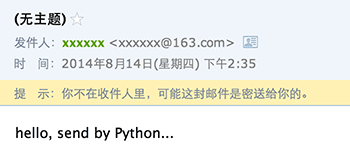
\includegraphics[width=0.6\linewidth]{fig/967446760519840.png}
\end{figure}


仔细观察,发现如下问题:

\begin{enumerate}
\def\labelenumi{\arabic{enumi}.}
\item
  邮件没有主题;
\item
  收件人的名字没有显示为友好的名字,比如\texttt{Mr\ Green\ \textless{}green@example.com\textgreater{}};
\item
  明明收到了邮件,却提示不在收件人中。
\end{enumerate}

这是因为邮件主题、如何显示发件人、收件人等信息并不是通过 SMTP 协议发给
MTA,而是包含在发给 MTA
的文本中的,所以,我们必须把\texttt{From}、\texttt{To}和\texttt{Subject}添加到\texttt{MIMEText}中,才是一封完整的邮件:

\begin{pythoncode}
from email import encoders
from email.header import Header
from email.mime.text import MIMEText
from email.utils import parseaddr, formataddr

import smtplib
    
def _format_addr(s):
    name, addr = parseaddr(s)
    return formataddr((Header(name, 'utf-8').encode(), addr))

from_addr = input('From: ')
password = input('Password: ')
to_addr = input('To: ')
smtp_server = input('SMTP server: ')

msg = MIMEText('hello, send by Python...', 'plain', 'utf-8')
msg['From'] = _format_addr('Python爱好者 <%s>' % from_addr)
msg['To'] = _format_addr('管理员 <%s>' % to_addr)
msg['Subject'] = Header('来自SMTP的问候……', 'utf-8').encode()
    
server = smtplib.SMTP(smtp_server, 25)
server.set_debuglevel(1)
server.login(from_addr, password)
server.sendmail(from_addr, [to_addr], msg.as_string())
server.quit()
\end{pythoncode}

我们编写了一个函数\texttt{\_format\_addr()}来格式化一个邮件地址。注意不能简单地传入\texttt{name\ \textless{}addr@example.com\textgreater{}},因为如果包含中文,需要通过\texttt{Header}对象进行编码。

\texttt{msg{[}\textquotesingle{}To\textquotesingle{}{]}}接收的是字符串而不是
list,如果有多个邮件地址,用\texttt{,}分隔即可。

再发送一遍邮件,就可以在收件人邮箱中看到正确的标题、发件人和收件人:

 
 \begin{figure}[htp]
	\centering
	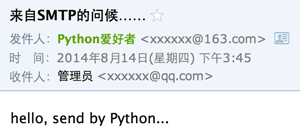
\includegraphics[width=0.6\linewidth]{fig/967453175707264.png}
\end{figure}


你看到的收件人的名字很可能不是我们传入的\texttt{管理员},因为很多邮件服务商在显示邮件时,会把收件人名字自动替换为用户注册的名字,但是其他收件人名字的显示不受影响。

如果我们查看 Email 的原始内容,可以看到如下经过编码的邮件头:

\begin{pythoncode}
From: =?utf-8?b?UHl0aG9u54ix5aW96ICF?= <xxxxxx@163.com>
To: =?utf-8?b?566h55CG5ZGY?= <xxxxxx@qq.com>
Subject: =?utf-8?b?5p2l6IeqU01UUOeahOmXruWAmeKApuKApg==?=
\end{pythoncode}

这就是经过\texttt{Header}对象编码的文本,包含 utf-8 编码信息和 Base64
编码的文本。如果我们自己来手动构造这样的编码文本,显然比较复杂。

\hypertarget{ux53d1ux9001-html-ux90aeux4ef6}{%
\subsubsection{发送 HTML 邮件}\label{ux53d1ux9001-html-ux90aeux4ef6}}

如果我们要发送 HTML
邮件,而不是普通的纯文本文件怎么办?方法很简单,在构造\texttt{MIMEText}对象时,把
HTML
字符串传进去,再把第二个参数由\texttt{plain}变为\texttt{html}就可以了:

\begin{pythoncode}
msg = MIMEText('<html><body><h1>Hello</h1>' +
    '<p>send by <a href="http://www.python.org">Python</a>...</p>' +
    '</body></html>', 'html', 'utf-8')
\end{pythoncode}

再发送一遍邮件,你将看到以 HTML 显示的邮件:

 
 \begin{figure}[htp]
	\centering
	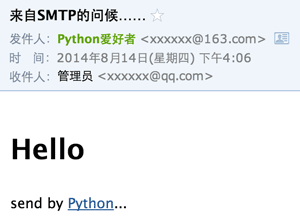
\includegraphics[width=0.6\linewidth]{fig/967455607327072.png}
\end{figure}


\hypertarget{ux53d1ux9001ux9644ux4ef6}{%
\subsubsection{发送附件}\label{ux53d1ux9001ux9644ux4ef6}}

如果 Email
中要加上附件怎么办?带附件的邮件可以看做包含若干部分的邮件:文本和各个附件本身,所以,可以构造一个\texttt{MIMEMultipart}对象代表邮件本身,然后往里面加上一个\texttt{MIMEText}作为邮件正文,再继续往里面加上表示附件的\texttt{MIMEBase}对象即可:

\begin{pythoncode}
msg = MIMEMultipart()
msg['From'] = _format_addr('Python爱好者 <%s>' % from_addr)
msg['To'] = _format_addr('管理员 <%s>' % to_addr)
msg['Subject'] = Header('来自SMTP的问候……', 'utf-8').encode()
msg.attach(MIMEText('send with file...', 'plain', 'utf-8'))
with open('/Users/michael/Downloads/test.png', 'rb') as f:
    
    mime = MIMEBase('image', 'png', filename='test.png')
    
    mime.add_header('Content-Disposition', 'attachment', filename='test.png')
    mime.add_header('Content-ID', '<0>')
    mime.add_header('X-Attachment-Id', '0')
    
    mime.set_payload(f.read())
    
    encoders.encode_base64(mime)
    
    msg.attach(mime)
\end{pythoncode}

然后,按正常发送流程把\texttt{msg}(注意类型已变为\texttt{MIMEMultipart})发送出去,就可以收到如下带附件的邮件:

 
 \begin{figure}[htp]
	\centering
	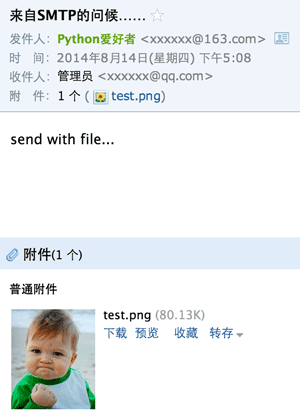
\includegraphics[width=0.6\linewidth]{fig/967464310443456.png}
\end{figure}


\hypertarget{ux53d1ux9001ux56feux7247}{%
\subsubsection{发送图片}\label{ux53d1ux9001ux56feux7247}}

如果要把一个图片嵌入到邮件正文中怎么做?直接在 HTML
邮件中链接图片地址行不行?答案是,大部分邮件服务商都会自动屏蔽带有外链的图片,因为不知道这些链接是否指向恶意网站。

要把图片嵌入到邮件正文中,我们只需按照发送附件的方式,先把邮件作为附件添加进去,然后,在
HTML
中通过引用\texttt{src="cid:0"}就可以把附件作为图片嵌入了。如果有多个图片,给它们依次编号,然后引用不同的\texttt{cid:x}即可。

把上面代码加入\texttt{MIMEMultipart}的\texttt{MIMEText}从\texttt{plain}改为\texttt{html},然后在适当的位置引用图片:

\begin{pythoncode}
msg.attach(MIMEText('<html><body><h1>Hello</h1>' +
    '<p><img src="cid:0"></p>' +
    '</body></html>', 'html', 'utf-8'))
\end{pythoncode}

再次发送,就可以看到图片直接嵌入到邮件正文的效果:

 
 \begin{figure}[htp]
	\centering
	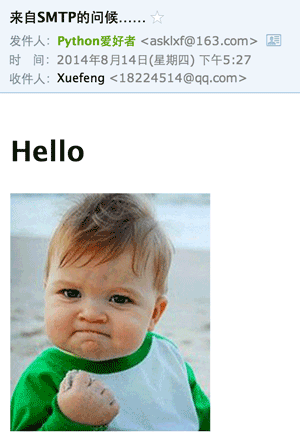
\includegraphics[width=0.6\linewidth]{fig/967488004941504.png}
\end{figure}


\hypertarget{ux540cux65f6ux652fux6301-html-ux548c-plain-ux683cux5f0f}{%
\subsubsection{同时支持 HTML 和 Plain
格式}\label{ux540cux65f6ux652fux6301-html-ux548c-plain-ux683cux5f0f}}

如果我们发送 HTML 邮件,收件人通过浏览器或者 Outlook
之类的软件是可以正常浏览邮件内容的,但是,如果收件人使用的设备太古老,查看不了
HTML 邮件怎么办?

办法是在发送 HTML 的同时再附加一个纯文本,如果收件人无法查看 HTML
格式的邮件,就可以自动降级查看纯文本邮件。

利用\texttt{MIMEMultipart}就可以组合一个 HTML 和 Plain,要注意指定
subtype 是\texttt{alternative}:

\begin{pythoncode}
msg = MIMEMultipart('alternative')
msg['From'] = ...
msg['To'] = ...
msg['Subject'] = ...

msg.attach(MIMEText('hello', 'plain', 'utf-8'))
msg.attach(MIMEText('<html><body><h1>Hello</h1></body></html>', 'html', 'utf-8'))
# 正常发送msg对象...
\end{pythoncode}

\hypertarget{ux52a0ux5bc6-smtp}{%
\subsubsection{加密 SMTP}\label{ux52a0ux5bc6-smtp}}

使用标准的 25 端口连接 SMTP
服务器时,使用的是明文传输,发送邮件的整个过程可能会被窃听。要更安全地发送邮件,可以加密
SMTP 会话,实际上就是先创建 SSL 安全连接,然后再使用 SMTP 协议发送邮件。

某些邮件服务商,例如 Gmail,提供的 SMTP
服务必须要加密传输。我们来看看如何通过 Gmail 提供的安全 SMTP 发送邮件。

必须知道,Gmail 的 SMTP 端口是 587,因此,修改代码如下:

\begin{pythoncode}
smtp_server = 'smtp.gmail.com'
smtp_port = 587
server = smtplib.SMTP(smtp_server, smtp_port)
server.starttls()

server.set_debuglevel(1)
...
\end{pythoncode}

只需要在创建\texttt{SMTP}对象后,立刻调用\texttt{starttls()}方法,就创建了安全连接。后面的代码和前面的发送邮件代码完全一样。

如果因为网络问题无法连接 Gmail 的 SMTP
服务器,请相信我们的代码是没有问题的,你需要对你的网络设置做必要的调整。

\hypertarget{ux5c0fux7ed3}{%
\subsubsection{小结}\label{ux5c0fux7ed3}}

使用 Python 的 smtplib
发送邮件十分简单,只要掌握了各种邮件类型的构造方法,正确设置好邮件头,就可以顺利发出。

构造一个邮件对象就是一个\texttt{Messag}对象,如果构造一个\texttt{MIMEText}对象,就表示一个文本邮件对象,如果构造一个\texttt{MIMEImage}对象,就表示一个作为附件的图片,要把多个对象组合起来,就用\texttt{MIMEMultipart}对象,而\texttt{MIMEBase}可以表示任何对象。它们的继承关系如下:

\begin{pythoncode}
Message
+- MIMEBase
   +- MIMEMultipart
   +- MIMENonMultipart
      +- MIMEMessage
      +- MIMEText
      +- MIMEImage
\end{pythoncode}

这种嵌套关系就可以构造出任意复杂的邮件。你可以通过
\href{https://docs.python.org/3/library/email.mime.html}{email.mime
文档}查看它们所在的包以及详细的用法。

\hypertarget{ux53c2ux8003ux6e90ux7801}{%
\subsubsection{参考源码}\label{ux53c2ux8003ux6e90ux7801}}

\href{https://github.com/michaelliao/learn-python3/blob/master/samples/mail/send_mail.py}{send\_mail.py}

